\chapter{Basic concepts}
\label{chap:basic-concepts}

In this chapter, we will introduce DortDB, the software that was written as a part of this thesis. DortDB is a TypeScript framework for querying existing in-memory data. It aims to be as configurable and modular as possible. It does not come with any query language by default -- the languages come in the form of plugins. Each language can then use the same already present building blocks, including a query optimizer or secondary indices. DortDB supports combining multiple languages in a single query, a concept more elaborated in chapter \ref{chap:multilang-queries}. We have already implemented three languages: SQL, XQuery, and Cypher. DortDB offers freedom in querying any kind of data using any kind of language, as long as a suitable data adapter is provided. DortDB will be released as an open-source library on NPM\footnote{\url{https://www.npmjs.com/}} (Node.js package manager).

Additionally, we have developed a graphical user interface for DortDB. It can be used to experiment with query optimizer strategies, inspect logical query plans, or query data.

\begin{figure}[!h]
    \centering
    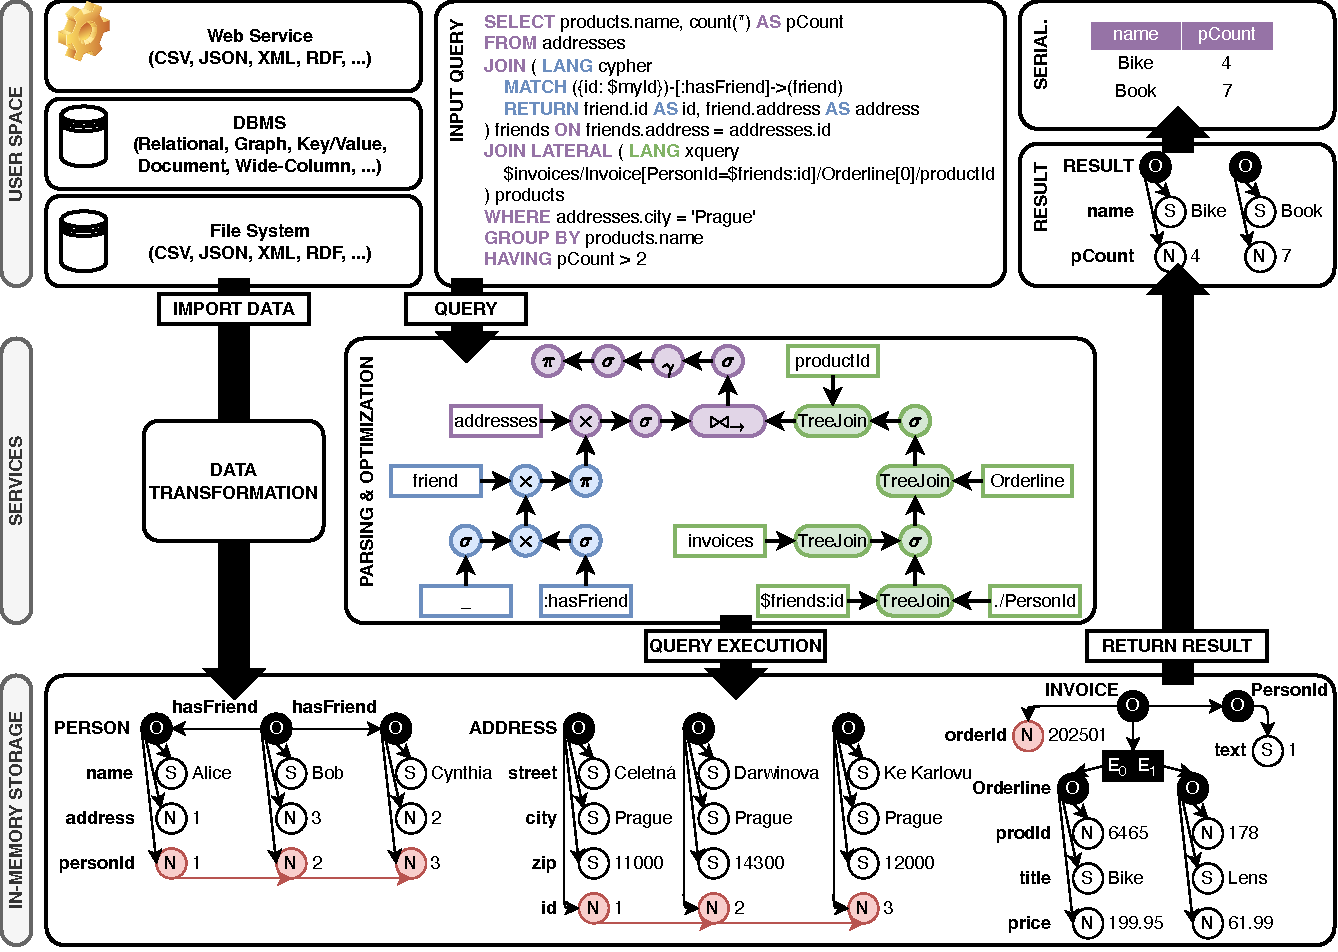
\includegraphics[width=\linewidth]{img/dortDB-workflow.pdf}
    \caption{Data import and query evaluation workflow in DortDB. The diagram was created by Pavel Koupil and comes from a demo paper accepted to the 51\textsuperscript{st} VLDB conference, which the author of this thesis coauthored with Pavel Koupil, Michal Kopecký, Jáchym Bártík, and Irena Holubová, but which has not yet been published at the time of writing.}
\end{figure}
